\chapter{Vector Spaces}

\section{The axioms}

Polynomials, matrices and functions can be added and scaled just like vectors in $\R^n$, and all the
theory of span, independence and bases carries over. We abstract the ten properties of Chapter 1.

\begin{definition}[Vector space]
A \emph{(real) vector space} is a set $\mathbb{V}$ with an operation of addition $\vec x+\vec y$ and scalar
multiplication $c\vec x$ ($c\in\R$) such that for all $\vec x,\vec y,\vec z\in\mathbb{V}$ and $c,d\in\R$:
\begin{enumerate}[label=V\arabic*.]
  \item $\vec x+\vec y\in\mathbb{V}$;
  \item $(\vec x+\vec y)+\vec z=\vec x+(\vec y+\vec z)$;
  \item $\vec x+\vec y=\vec y+\vec x$;
  \item there is an element $\vec 0\in\mathbb{V}$ (the \emph{zero vector}) with $\vec x+\vec 0=\vec x$ for all $\vec x$;
  \item for each $\vec x$ there is $-\vec x\in\mathbb{V}$ (the \emph{additive inverse}) with $\vec x+(-\vec x)=\vec 0$;
  \item $c\vec x\in\mathbb{V}$;
  \item $c(d\vec x)=(cd)\vec x$;
  \item $(c+d)\vec x=c\vec x+d\vec x$;
  \item $c(\vec x+\vec y)=c\vec x+c\vec y$;
  \item $1\vec x=\vec x$.
\end{enumerate}
Elements of $\mathbb{V}$ are called \emph{vectors}, whatever they actually are.
\end{definition}

\begin{example}[Standard examples]
\begin{itemize}
  \item $\R^n$.
  \item $\Poly{n}$: polynomials $a_0+a_1x+\dots+a_nx^n$ of degree at most $n$, with the usual addition and scalar
        multiplication of polynomials. The zero vector is the zero polynomial.
  \item $\Mat{m}{n}$: $m\times n$ matrices with entrywise operations; zero vector $O_{m,n}$.
  \item $\mathcal{F}(a,b)$: all functions $f:(a,b)\to\R$, with $(f+g)(x)=f(x)+g(x)$ and $(cf)(x)=cf(x)$. The
        zero vector is the function that is identically $0$. Subspaces include continuous functions
        $C(a,b)$ and differentiable functions.
  \item The trivial vector space $\{\vec 0\}$.
\end{itemize}
\end{example}

\begin{example}[A strange vector space]
Let $\mathbb{V}=\{x\in\R:x>0\}$ with ``addition'' $x\oplus y=xy$ and ``scalar multiplication''
$c\odot x=x^c$. Then $\mathbb{V}$ is a vector space: e.g.\ V4 holds with zero vector $1$ (since $x\oplus1=x$),
V5 with $-x = 1/x$, and V8 is $x^{c+d}=x^cx^d=(c\odot x)\oplus(d\odot x)$. The axioms only care about how
the operations behave, not what they look like.
\end{example}

\begin{theorem}
In any vector space: $0\vec x=\vec0$, $(-1)\vec x=-\vec x$, $c\vec 0=\vec 0$; the zero vector and additive inverses are
unique.
\end{theorem}
\begin{proof}[Proof of $0\vec x=\vec 0$]
$0\vec x=(0+0)\vec x=0\vec x+0\vec x$ by V8. Adding $-(0\vec x)$ to both sides and using V2, V5, V4 gives
$\vec 0=0\vec x$.
\end{proof}

\section{Subspaces}

\begin{definition}
A subset $\mathbb{S}$ of a vector space $\mathbb{V}$ is a \emph{subspace} if it is a vector space under the same
operations.
\end{definition}

\begin{theorem}[Subspace Test]
$\mathbb{S}\subseteq\mathbb{V}$ is a subspace iff $\mathbb{S}$ is non-empty and closed under addition and scalar
multiplication.
\end{theorem}

\begin{example}
The symmetric matrices $\mathbb{S}=\{A\in\Mat{2}{2}:A^T=A\}$ form a subspace: $O^T=O$; and
$(A+B)^T=A^T+B^T=A+B$, $(cA)^T=cA^T=cA$.
\end{example}

\begin{example}
$\mathbb{S}=\{p\in\Poly{2}:p(1)=0\}$ is a subspace: the zero polynomial vanishes at $1$, and
$(p+q)(1)=0+0$, $(cp)(1)=c\cdot0$. But $\{p\in\Poly{2}:p(1)=1\}$ is not (it does not contain $0$), and
neither is the set of polynomials of degree \emph{exactly} $2$ ($x^2+(-x^2)=0$ has degree less than 2).
\end{example}

\begin{example}
The invertible $2\times2$ matrices do not form a subspace of $\Mat22$: $I$ and $-I$ are invertible but $I+(-I)=O$ is not.
\end{example}

\section{Span and linear independence}

Definitions of linear combination, $\Span$, linear (in)dependence, spanning set and basis are word-for-word the
same as in $\R^n$. Span is always a subspace. The difference is computational: we must translate
problems about polynomials or matrices into systems of equations by comparing coefficients.

\begin{example}
Is $\{1+x+x^2,\ 1+2x+3x^2,\ 2+3x+4x^2\}$ linearly independent in $\Poly{2}$? Suppose
$c_1(1+x+x^2)+c_2(1+2x+3x^2)+c_3(2+3x+4x^2)=0$. Comparing the coefficients of $1,x,x^2$:
\[
\left[\begin{array}{ccc|c}1&1&2&0\\1&2&3&0\\1&3&4&0\end{array}\right]
\xrightarrow{\substack{R_2-R_1\\R_3-R_1}}
\left[\begin{array}{ccc|c}1&1&2&0\\0&1&1&0\\0&2&2&0\end{array}\right]
\xrightarrow{R_3-2R_2}
\left[\begin{array}{ccc|c}1&1&2&0\\0&1&1&0\\0&0&0&0\end{array}\right].
\]
$c_3$ is free, so there are non-trivial solutions: the set is dependent. Taking $c_3=-1$: $c_2=1$, $c_1=1$, i.e.\
$(1+x+x^2)+(1+2x+3x^2)=2+3x+4x^2$.
\end{example}

\begin{example}
Is $\begin{bmatrix}1&2\\3&4\end{bmatrix}$ in $\Span\left\{\begin{bmatrix}1&0\\1&0\end{bmatrix},\begin{bmatrix}0&1\\0&1\end{bmatrix},\begin{bmatrix}1&1\\0&0\end{bmatrix}\right\}$?
We need $c_1+c_3=1$, $c_2+c_3=2$, $c_1=3$, $c_2=4$ (entries $(1,1),(1,2),(2,1),(2,2)$). Then
$c_3=1-3=-2$ and $c_3=2-4=-2$: consistent. So yes, with $(c_1,c_2,c_3)=(3,4,-2)$.
\end{example}

\begin{example}[Functions]
$\{\sin x,\cos x\}$ is linearly independent in $\mathcal F(\R)$: if $c_1\sin x+c_2\cos x=0$ for \emph{all}
$x$, then $x=0$ gives $c_2=0$ and $x=\pi/2$ gives $c_1=0$. (Note that the equation must hold as functions, i.e.\
at every $x$.)
\end{example}

Functions add pointwise, just like vectors add componentwise; here $\sin x + \cos x$ is a vector
in $\Span\{\sin x,\cos x\}$:
\begin{center}
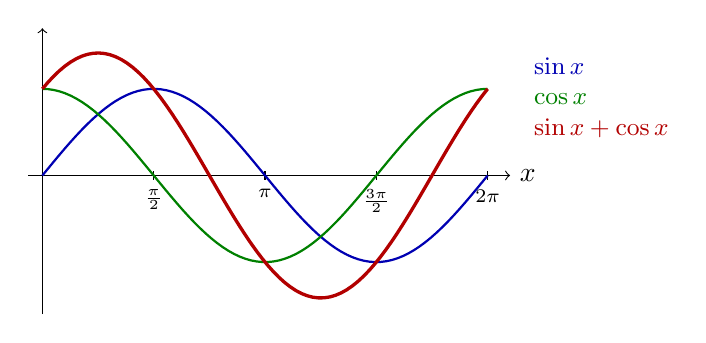
\begin{tikzpicture}[x=0.9cm,y=1.1cm]
  \draw[->] (-0.2,0) -- (6.6,0) node[right] {$x$};
  \draw[->] (0,-1.6) -- (0,1.7);
  \foreach \t/\l in {1.5708/{\frac\pi2},3.1416/{\pi},4.7124/{\frac{3\pi}2},6.2832/{2\pi}} { \draw (\t,0.05) -- (\t,-0.05) node[below,font=\scriptsize] {$\l$}; }
  \draw[thick,blue!70!black,domain=0:6.2832,samples=80] plot (\x,{sin(\x r)});
  \draw[thick,green!50!black,domain=0:6.2832,samples=80] plot (\x,{cos(\x r)});
  \draw[very thick,red!70!black,domain=0:6.2832,samples=80] plot (\x,{sin(\x r)+cos(\x r)});
  \node[font=\small,align=left,right] at (6.8,0.9) {{\color{blue!70!black}$\sin x$}\\{\color{green!50!black}$\cos x$}\\{\color{red!70!black}$\sin x + \cos x$}};
\end{tikzpicture}
\end{center}

\section{Bases and dimension}

\begin{theorem}[Replacement / Exchange Lemma]
If $\{\vec v_1,\dots,\vec v_n\}$ spans $\mathbb V$ and $\{\vec u_1,\dots,\vec u_k\}\subseteq\mathbb V$ is linearly
independent, then $k\le n$.
\end{theorem}
\begin{proof}[Proof sketch]
Write $\vec u_j=\sum_i a_{ij}\vec v_i$. If $k>n$, the homogeneous system $A\vec c=\vec 0$ ($A=[a_{ij}]$ is $n\times k$)
has a non-trivial solution, and then $\sum_jc_j\vec u_j=\sum_i(\sum_ja_{ij}c_j)\vec v_i=\vec 0$, contradicting
independence.
\end{proof}

\begin{definition}[Dimension]
If $\mathbb V$ has a basis with $n$ vectors, then (by the lemma) every basis has $n$ vectors, and
$\dim\mathbb V=n$; $\mathbb V$ is \emph{finite-dimensional}. $\dim\{\vec0\}=0$. If no finite set spans
$\mathbb V$, it is \emph{infinite-dimensional} (e.g.\ $\mathcal F(\R)$, or the space of all polynomials).
\end{definition}

\begin{example}
$\dim\R^n=n$; $\dim\Poly{n}=n+1$ (standard basis $\{1,x,\dots,x^n\}$); $\dim\Mat mn=mn$ (standard basis
$\{E_{ij}\}$ with a single $1$ in position $(i,j)$). The symmetric $2\times2$ matrices have basis
$\left\{\begin{bmatrix}1&0\\0&0\end{bmatrix},\begin{bmatrix}0&1\\1&0\end{bmatrix},\begin{bmatrix}0&0\\0&1\end{bmatrix}\right\}$, dimension $3$.
\end{example}

\begin{example}
Find a basis and the dimension of $\mathbb S=\{p\in\Poly2:p(1)=0\}$. Writing $p=a+bx+cx^2$, the condition is
$a+b+c=0$, i.e.\ $a=-b-c$, so
$p=-b-c+bx+cx^2=b(x-1)+c(x^2-1)$. Thus $\mathbb S=\Span\{x-1,x^2-1\}$, and this set is independent (neither is a
multiple of the other). So $\dim\mathbb S=2$.
\end{example}

\begin{theorem}
Let $\dim\mathbb V=n$.
\begin{enumerate}
  \item Any set of more than $n$ vectors is dependent; any set of fewer than $n$ vectors does not span.
  \item A set of exactly $n$ vectors is a basis iff it is independent iff it spans (``two out of three'').
  \item Every independent set can be extended to a basis; every spanning set contains a basis.
  \item If $\mathbb S$ is a subspace, $\dim\mathbb S\le n$, with equality iff $\mathbb S=\mathbb V$.
\end{enumerate}
\end{theorem}
\begin{proof}[Proof sketch of (3)]
If an independent set $B$ does not span, pick $\vec v\notin\Span B$; then $B\cup\{\vec v\}$ is still independent
(a relation with non-zero coefficient on $\vec v$ would put $\vec v$ in $\Span B$). This stops after at most $n$ steps by
(1). For a spanning set, repeatedly remove a vector that is a combination of the others (Chapter 1).
\end{proof}

\begin{example}
Extend $\{1+x,\ 1-x\}$ to a basis of $\Poly2$. Since $\dim\Poly2=3$, we need one more vector not in their
span. Every combination $a(1+x)+b(1-x)$ has no $x^2$ term, so $x^2$ works: $\{1+x,1-x,x^2\}$ is independent, hence a
basis by ``two out of three''.
\end{example}

\section{Coordinates}

\begin{definition}
Let $\mathcal B=\{\vec v_1,\dots,\vec v_n\}$ be an (ordered) basis of $\mathbb V$. For $\vec x\in\mathbb V$, write
uniquely $\vec x=c_1\vec v_1+\dots+c_n\vec v_n$. The \emph{coordinate vector} of $\vec x$ with respect to $\mathcal B$ is
\[
  [\vec x]_{\mathcal B}=\begin{bmatrix}c_1\\\vdots\\c_n\end{bmatrix}\in\R^n .
\]
\end{definition}

\begin{theorem}
The coordinate map is linear: $[b\vec x+c\vec y]_{\mathcal B}=b[\vec x]_{\mathcal B}+c[\vec y]_{\mathcal B}$. Moreover
$\{\vec x_1,\dots,\vec x_k\}$ is independent (spans $\mathbb V$) iff $\{[\vec x_1]_{\mathcal B},\dots,[\vec x_k]_{\mathcal B}\}$ is
independent (spans $\R^n$).
\end{theorem}

This is why comparing coefficients worked in the examples above: we were really computing in $\R^n$ via
coordinates with respect to the standard basis.

\begin{center}
\begin{tikzpicture}[>={Stealth}]
  \node[draw,rounded corners,minimum width=3.2cm,minimum height=1.6cm,align=center,fill=blue!8] (V) at (0,0)
    {$\Poly 2$\\[2pt]\small $3 + x + 2x^2$};
  \node[draw,rounded corners,minimum width=3.2cm,minimum height=1.6cm,align=center,fill=green!8] (R) at (6,0)
    {$\R^3$\\[2pt]\small $(2,1,2)$};
  \draw[->,thick] (V.20) -- node[above,font=\small] {$[\,\cdot\,]_{\mathcal B}$} (R.160);
  \draw[->,thick] (R.200) -- node[below,font=\small] {$c_1\vec v_1 + c_2\vec v_2 + c_3\vec v_3$} (V.340);
\end{tikzpicture}
\end{center}
With $\mathcal B = \{1+x,\ 1-x,\ x^2\}$ (as in the example below), taking coordinates turns a question
about polynomials into one about $\R^3$, and rebuilding from the coordinates goes back.

\begin{example}
Find $[p]_{\mathcal B}$ for $p=3+x+2x^2$ and $\mathcal B=\{1+x,\ 1-x,\ x^2\}$. Solve
$a(1+x)+b(1-x)+cx^2=3+x+2x^2$:
\[
\left[\begin{array}{ccc|c}1&1&0&3\\1&-1&0&1\\0&0&1&2\end{array}\right]
\xrightarrow{R_2-R_1}
\left[\begin{array}{ccc|c}1&1&0&3\\0&-2&0&-2\\0&0&1&2\end{array}\right]
\xrightarrow{-\frac12R_2}
\left[\begin{array}{ccc|c}1&1&0&3\\0&1&0&1\\0&0&1&2\end{array}\right]
\xrightarrow{R_1-R_2}
\left[\begin{array}{ccc|c}1&0&0&2\\0&1&0&1\\0&0&1&2\end{array}\right].
\]
So $[p]_{\mathcal B}=(2,1,2)$. Check: $2(1+x)+(1-x)+2x^2=3+x+2x^2$.
\end{example}

\begin{important}[Pitfall]
A coordinate vector depends on the \emph{order} of the basis vectors, and $[\vec x]_{\mathcal B}$ lives in $\R^n$
even when $\vec x$ is a polynomial or a matrix.
\end{important}

\section*{Summary}
\begin{itemize}
  \item A vector space is any set with $+$ and scalar multiplication satisfying V1--V10: $\R^n$, $\Poly n$,
        $\Mat mn$, function spaces.
  \item Subspace test: non-empty, closed under $+$ and scalar multiplication.
  \item Span, independence and bases work as in $\R^n$; reduce to linear systems by comparing coefficients.
  \item All bases have the same size $\dim\mathbb V$; $\dim\Poly n=n+1$, $\dim\Mat mn=mn$. With $n$ vectors,
        independent $\iff$ spanning.
  \item Coordinates $[\vec x]_{\mathcal B}\in\R^n$ turn any $n$-dimensional space into $\R^n$.
\end{itemize}
